\documentclass{pj}

\usepackage{hyperref}
\usepackage{cite}
\usepackage{amsmath}
%\interdisplaylinepenalty=2500 % suggested by IEEE to use with amsmath package
\usepackage{amsfonts}
\usepackage{graphicx}
\usepackage{subfigure}
\usepackage{epstopdf}

\usepackage[T1]{fontenc} % optional
\usepackage[cmintegrals]{newtxmath}
\usepackage{bm} % optional

% correct bad hyphenation here
\hyphenation{op-tical net-works semi-conduc-tor}

\begin{document}
\setcounter{page}{1}
\pjheader{}

\title{Design of High Speed Link System}
%\maketitle

\newcommand{\defaultfigurewidth}{0.5\columnwidth}

\footnote{\hskip-0.12in\textsuperscript{1} Chang-Pao Chang (cchang95@uiuc.edu)}
\footnote{\hskip-0.12in\textsuperscript{2} Xiou Ge (xiouge2@uiuc.com)}
\footnote{\hskip-0.12in*\ University of Illinois at Urbana-Champaign, Urbana, Illinois, 61801}

\author{Chang-Pao Chang\textsuperscript{*,1} and Xiou Ge\textsuperscript{*,2}}



\begin{abstract}
	
\end{abstract}
%
\section{introduction}
\label{sec:Intro}

\begin{figure}[htbp!]
	\centering
	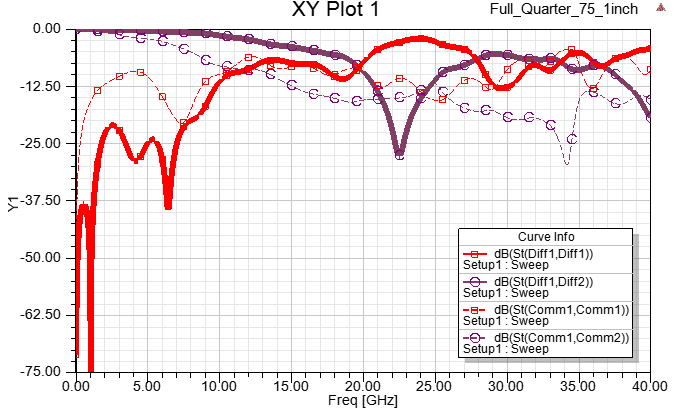
\includegraphics[width=0.8\columnwidth]{./img/PCB/Via_Transition/S_parameter.png}
	\caption{S parameter of via transition in PCB.}
	\label{fig:pcb_via_tran_S} % label must put at the last
\end{figure}


\section{Conclusion}
In this paper, we use the vector electric field formulation, combined with both edge and element basis, to analyze several type of waveguide structure. Both homogeneous and inhomogeneous  waveguide shows a good agreement to the analytic solution. In addition, the slow wave factors of MIS structure are analyzed with different substrate loss. The transitions from slow wave mode to quasi-TEM mode or skip-depth mode can be clearly observed. 

% =============  Reference Section ==============

%\bibliographystyle{IEEEtran}
%\bibliography{IEEEabrv,F:/SoftwarePC/AutoupdateZoteroLibrary}

%\begin{thebibliography}{99}	
%
%\end{thebibliography}


\end{document}

